\documentclass[11pt]{article}

\usepackage{setspace}
\usepackage{amsmath}
\usepackage{enumitem}
\usepackage{amsfonts} 
\usepackage{relsize}
\usepackage{graphicx}
\usepackage[top=2cm,bottom=2cm,left=2.5cm,right=2.5cm,marginparwidth=1.75cm]{geometry}
\setlength{\parindent}{0cm}

\def\lc{\left\lceil}   
\def\rc{\right\rceil}
\def\lf{\left\lfloor}   
\def\rf{\right\rfloor}

\title{4041 Homework 3}
\author{Fletcher Gornick}
\date{October 11, 2021}

\spacing{1.5}
\begin{document}
 \maketitle 

 \section*{8.1}
 \subsection*{8.1-1}
 \textbf{What is the smallest possible depth of a leaf in a decision tree for a comparison 
 sort?} \\

 The best  case for a comparison sort is when we have $n-1$ comparisons.  Each 
 node of a decision tree is represented as \texttt{i:j}, which compares the $ith$ element with 
 the $jth$ element of an array, where $1 \leq i$, $j \leq n$, and $n$ is the length of the array.
 The best path along this decision tree is one where we never reach a node \texttt{i:k} or 
 \texttt{k:j} after node \texttt{i:j} for some $k$ in the array not including $i$ or $j$.  An 
 example of this is when the array is already sorted, making $n-1$ pairs of relative ordering. 
 So this smallest possible depth of a decision tree for a comparison sort is $n-1$ for an array 
 of size $n$.
 \newpage

 \subsection*{8.1-3}
 \textbf{Show that there is no comparison sort whose running time is linear for at least half 
 of the $n!$ inputs of length $n$. What about a fraction of $1/n$ of the inputs of length $n$? 
 What about a fraction $1/2^n$?} \\

 We can represent comparison sort as a decision tree with $n!$ leaves representing all the 
 possible permutations of an array of size $n$.  This tree will be given height $h$ with $l$
 reachable leaves.  By the proof from theorem 8.1 in the textbook, we know $n! \leq l \leq 2^h$. 
 We also know that $n! \geq n!/2 \geq n!/n \geq n!/2^n$ for inputs of length $n \geq 2$, so it 
 follows that $2^h \geq n!/2^n$.  Since we know that $n!/2^n$ is the smallest number of outputs 
 that need to be reached in linear time for this problem, if we can show that this isn't possible, 
 then it follows that it's also not possible for fractions of $n!/2$ or $n!/n$.
 $$2^h \;\geq\; n!/2^n \;\;\Rightarrow\;\; h \;\geq\; \lg(n!/2^n) \;=\; \lg(n!) - \lg(2^n) \;=\; 
 \Theta (n \lg n) - n \;=\; \Theta (n \lg n)$$
 Again, since $n!/2^n$ inputs can't be reached in linear time, then neither can $n!/2$ inputs, or 
 $n!/n$ inputs.
 So, in conclusion, a comparison tree with leave representing the $n!$ possible permutations of an 
 array of length $n$ has less than $n!/2$ leaves with a depth linearly proportional to the array's 
 size $n$.  There are also less than $n!/n$ and $n!/2^n$ leaves of depth $n$ that represent a 
 permutation of this array.
 \newpage

 \subsection*{8.1-4}
 \textbf{Suppose that you are given a sequence of $n$ elements to sort. The input sequence 
 consists of $n/k$ subsequences, each containing $k$ elements. The elements in a given 
 subsequence are all smaller than the elements in the succeeding subsequence and larger than 
 the elements in the preceding subsequence. Thus, all that is needed to sort the whole 
 sequence of length $n$ is to sort the $k$ elements in each of the $n/k$ subsequences. Show 
 an $\Omega(n \lg k)$ lower bound on the number of comparisons needed to solve this variant 
 of the sorting problem. (\textit{Hint:} It is not rigorous to simply combine the lower bounds 
 for the individual subsequences).} \\

 This $n$ length sequence contains $n/k$ subsequences of length $k$.  These subsequences can have 
 any order, but the order between the subsequences are set.  So each subsequence has $k!$ 
 permutations, meaning that the number of permutations of the whole sequence is the number of 
 permutations of a subsequence multiplied by the number of permutations of the rest.  So we can 
 conclude that there are $(k!)^{n/k}$ possible permutations for these subsequences.  Therefore 
 our comparison tree must have $(k!)^{n/k}$ leaves.  In order for this to be the case, the tree 
 must have a certain height.  Since a perfect tree of height $h$ has $2^h$ leaves, we know that 
 $2^h \geq (k!)^{n/k}$, otherwise there won't be enough leaves to cover every possible permutation. 
 So we can solve for the height of our tree like so... 
 $$2^h \;\geq\; (k!)^{n/k} \;\;\Rightarrow\;\; h \;\geq\; \lg ((k!)^{n/k}) \;=\; \frac{n}{k} \lg (k!)
 \;\geq\; \frac{n}{k} \cdot k \lg k \;=\; n \lg k$$
 Since $h$ represents the number of comparisons needed to reach a permutation, and $h \geq n \lg k$, 
 we can conclude that there's an $\Omega(n \lg k)$ lower bound on the number of comparisons needed to 
 find the sorted permutation of this sequence.  Also the step where we converted $\lg (k!)$ to $k \lg k$
 is highlighted in page 58 of the book.
 \newpage

 \section*{9.2}
 \subsection*{9.2-3}
 \textbf{Write an iterative version of \texttt{randomized-select}.} \\
 \begin{verbatim}
 randomized-select(A,i)
     if (i >= A.length or i < 0) return "index out of range"

     j = i
     p = 0
     r = A.length - 1

     while (p < r) {
         q = randomized-partition(A,p,r)
         k = q - p + 1 
         
         if (j == k) return A[q]

         if (j < k) r = q-1

         if (j > k)
           p = q+1 
           j = j-k
     }
     return A[p]    // when and if p == r
 \end{verbatim}
 I'm assuming it's okay that we don't also need to write an iterative version of the 
 \texttt{randomized-partition} algorithm because it wasn't explicitly stated.
 \newpage

 \section*{9.3}
 \subsection*{9.3-3}
 \textbf{Show how quicksort can be made to run in $O(n \lg n)$ time in the worst case, assuming 
 that all elements are distinct.} \\

 In section 9.3 of the textbook, it is shown that we can calculate the $i$th smallest value of an 
 input array in $O(n)$ time.  This technique can be used to find the median in $O(n)$ time as well 
 This is done by dividing the $n$ elements of the array into $\lf n/5 \rf$ subarrays of length 5.  
 Then, using insertion sort, we can pick the median out of all the subarrays, then recursively call 
 select to find that median.  It's been proved that this can be done in $O(n)$ time in the textbook 
 so I won't elaborate further on that matter. \\ 

 A normal quicksort algorithm just calls partition, then recursively calls quicksort on the 2 smaller 
 partitioned arrays.  This can be $O(n^2)$ if the array is partitioned in a bad place.  We can keep 
 this from happening by calling the select algorithm, to find the median value of the array in $O(n)$ 
 time.  Thus the two following recursive calls to quickselect are always done on an array that's half 
 the size.  So we can write this new reccurance relation like so...

 \[
   T(n) = 
   \begin{cases}
     O(1) & \text{if } n = 1, \\
     2T(n/2) + O(n) & \text{if } n > 1
   \end{cases}
 \]

 The $2T(n/2)$ is from the two recursive calls to quicksort.  Again we know that the recursive call 
 will be on an array with half the size because our select algorithm found the median.  The $O(n)$ 
 is from two things.  The first is our select algorithm, which finds the median in $O(n)$ time.  And 
 the second is from a call to partition, which must iterate through the array once, to move the 
 elements around, so our pivot ends in the right spot with all the values smaller than it below, and 
 all the values greater than it above.  Since the array is only looped through once, this is an 
 additional $O(n)$ time complexity, which is just added onto the $O(n)$ complexity from the select 
 algorithm. \\

 This recurrance relation is $O(n\lg n)$. I used induction to prove this relation is $O(n \lg n)$ on 
 my previous homework, question 2.3-3, so I won't recreate the proof.
 \newpage


 \subsection*{9.3-5}
 \textbf{Suppose that you have a “black-box” worst-case linear-time median subroutine. Give a 
 simple, linear-time algorithm that solves the selection problem for an arbitrary order 
 statistic.} \\

 We can first use the median algorithm which is linear.  Then we can partition the array around 
 that median element, which is also linear.  There are 3 cases we need to look at in order to 
 select the correct element. Suppose the index we're looking for is represented as $i$. \\

 The first (best possible) case is if the median we found is partitioned at position $i$, then we 
 can just return the median. \\

 The second case is if our median is in a higher position.  Then we can recursively call our selection 
 algorithm on the bottom half of the array. \\

 The final case is if the median is below position $i$. For this we must alter the value of $i$ to 
 subtract off the length of the first half of the array, then recursively call the selection algorithm 
 to look for the new $i$ index. The algorithm would look something like this...\\

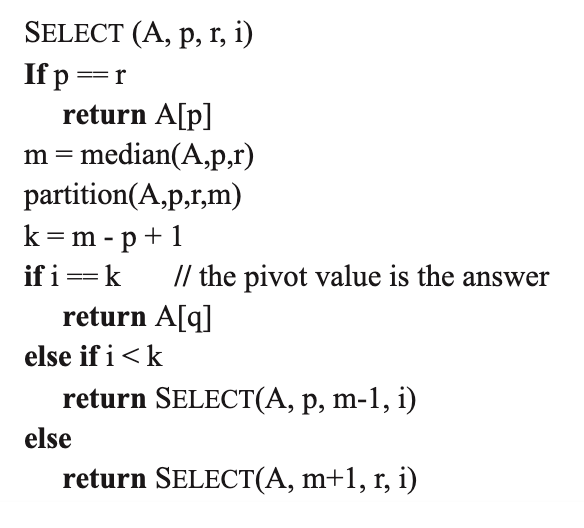
\includegraphics[scale=0.8]{select.png}

I made this image myself but just formatted it similar to the \texttt{RANDOMIZED-SELECT} function in 
9.2 of the textbook.  Also the last else statement where I call \texttt{SELECT}, it should be $i-k$ as 
the last parameter, not $i$.
 \newpage

 \section*{21.3}
 \subsection*{21.3-2}
 \textbf{Write a nonrecursive version of \texttt{find-set} with path compression.}
 \begin{verbatim}
   if (x == x.p) return x               \\ element is already the root
   else if (x.p.p == x.p) return x.p    \\ element already directly connected to root
   else 
     root = x
     while (root != root.p) root = root.p   \\ find root node of set
     while (x != x.p)                   \\ connect nodes to root node and go up
       tmp = x.p                        \\ the set until reaching root
       x.p = root                       \\ tmp keeps track of parent node
       x = tmp 
    return root
 \end{verbatim}

\end{document}
